\documentclass[crop,tikz]{standalone}

\tikzset{>=latex}

\begin{document}
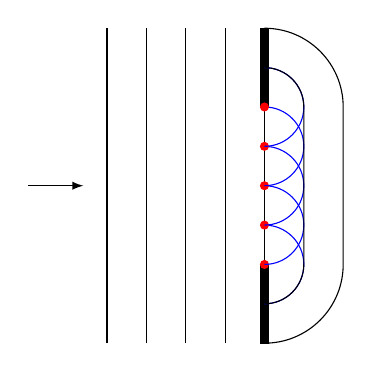
\begin{tikzpicture}
  \foreach\X in {-2,-1.5,-1,-0.5,0} {\draw(\X,-2)--(\X,2);}
  \draw[->] (-3,0) -- +(0.7,0);
  \draw[fill] (0.05,-2) rectangle (-0.05,-1);
  \draw[fill] (0.05,2)  rectangle (-0.05,1);
  \foreach\Y in {-1,-0.5,...,1} {%
    \draw[fill,red] (0,\Y) circle (0.05);
    \draw[blue] (0,\Y)+(-90:0.5) arc (-90:+90:0.5);
  }
  \draw (0,-1.5) arc (-90:0:0.5) -- (0.5,1) arc (0:90:0.5);
  \draw (0,-2)   arc (-90:0:1)   -- (1,1)   arc (0:90:1);
\end{tikzpicture}
\end{document}
